
\section{Ambiguities in ICA and limitations}
\begin{frame}{\secname}

Sources can be recovered up to:
\begin{itemize}
\item sign
\item scale
\item permutation i.e. ordering
\item only one gaussian distributed source
\end{itemize}
\begin{align*}
\vec P &:= \text{arbitrary permutation matrix}\\
\vec \Lambda &:= \text{arbitrary diagonal matrix}
\end{align*}
\begin{align}
\vec x &= \vec A \, \vec s\\
\vec x &= \lbrack \, \vec A\, \vec P^{-1} \vec \Lambda^{-1}\, \rbrack \, \lbrack \, \vec \Lambda \, \vec P \, \vec s\, \rbrack
\end{align}

\end{frame}

\notesonly{
ICA cannot resolve if the mixing matrix is $\vec A$ or a permuted and/or scaled version of $\vec A$.
It can \textbf{also} not resolve if the independent sources are $\vec s$ or a permuted and/or scaled version of $\vec s$.
}

\begin{frame}{\secname}

Permutations and scaling are not an issue for ICA because permutation and scaling do not interfere with statistical independence.

\begin{equation}
P_{s_1, s_2}(\widehat {\vec s}) \eqexcl  P_{s_1} (\widehat{s}_1) \cdot P_{s_2} (\widehat{s}_2)
\end{equation}

\slidesonly{
\begin{center}
	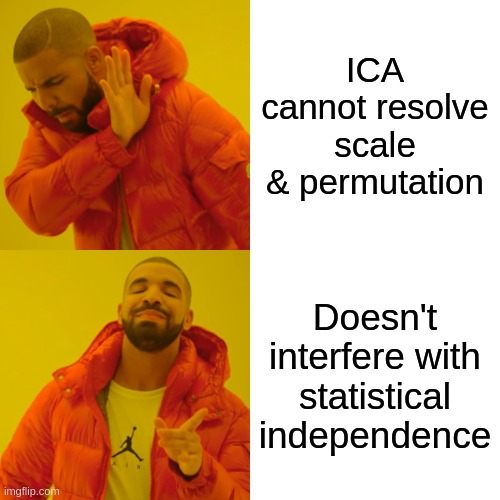
\includegraphics[width=0.4\textwidth]{img/meme_doesnotinterfere}%
\end{center}
}

\end{frame}

\notesonly{
We can verify that ambiguities to scale and permutation do not interfere with statistical independence.
}

\begin{frame}{Verification}
Permutations of sources
{\footnotesize
\begin{equation}
	\arraycolsep=1.4pt%\def\arraystretch{2.2}
	\begin{array}{ccc}
	\left( \begin{array}{ll}
		\textcolor{gray}{\widehat{s}_1} \\ \widehat{s}_2
	\end{array} \right)
	=
	\left( \begin{array}{ll}
	\textcolor{gray}{\mathrm{w}_{11}} & \textcolor{gray}{\mathrm{w}_{12}} \\
		\mathrm{w}_{21} & \mathrm{w}_{22} 
	\end{array} \right)
	\left( \begin{array}{ll}
		\mathrm{x}_1 \\ \mathrm{x}_2
	\end{array} \right)
	& \corresponds &
	\left( \begin{array}{ll}
		\widehat{s}_2 \\ \textcolor{gray}{\widehat{s}_1}
	\end{array} \right)
	 = 
	\left( \begin{array}{ll}
		\mathrm{w}_{21} & \mathrm{w}_{22} \\
		\textcolor{gray}{\mathrm{w}_{11}} & \textcolor{gray}{\mathrm{w}_{12}} 
	\end{array} \right)
	\left( \begin{array}{ll}
		\mathrm{x}_1 \\ \mathrm{x}_2
	\end{array} \right)
	\\\\
	P_{s_1} (\widehat{s}_1) \cdot P_{s_2} (\widehat{s}_2)
	&& 
	P_{s_2} (\widehat{s}_2) \cdot P_{s_1} (\widehat{s}_1)
	\end{array}
\end{equation}
}
%%%%%%%%%%%%%%%%%%%%%%%%%%%%%%%%%%%%%%%%%%%%%%%%%%%%%%%%%%%%%%%%%%%
Scaling of source amplitudes:

{\footnotesize
\begin{equation}
	\begin{array}{ccc}
	\arraycolsep=1.4pt
	\left( \begin{array}{ll}
		\widehat{s}_1 \\ \widehat{s}_2
	\end{array} \right)
	=
	\left( \begin{array}{ll}
		\mathrm{w}_{11} & \mathrm{w}_{12} \\
		\mathrm{w}_{21} & \mathrm{w}_{22} 
	\end{array} \right)
	\left( \begin{array}{ll}
		\mathrm{x}_1 \\ \mathrm{x}_2
	\end{array} \right)
	& \corresponds &
	\left( \begin{array}{ll}
		\textcolor{gray}{a}\,\widehat{s}_1 \\ 
                 \textcolor{gray}{b}\,\widehat{s}_2
	\end{array} \right)
	=
	\left( \begin{array}{ll}
		\textcolor{gray}{a}\,\mathrm{w}_{11} & \textcolor{gray}{a}\,\mathrm{w}_{12} \\
		\textcolor{gray}{b}\,\mathrm{w}_{21} & \textcolor{gray}{b}\,\mathrm{w}_{22} 
	\end{array} \right)
	\left( \begin{array}{ll}
		\mathrm{x}_1 \\ \mathrm{x}_2
	\end{array} \right)
	\\\\
	P_{s_1} (\widehat{s}_1) \cdot P_{s_2} (\widehat{s}_2)
	&& 
	aP_{s_1} (a\widehat{s}_1) \cdot bP_{s_2} (b\, \widehat{s}_2)
	\end{array}
\end{equation}
}
\end{frame}

\subsection{Implications of the ambiguities}

\begin{frame}{\subsecname}

We can assume:
\begin{equation}
\E \lbrack \, \vec s \, \rbrack = \vec 0
\end{equation}

Subtracting the mean from $\vec x$ does not change $\vec A$:

\begin{equation}
\vec x - \E \lbrack \, \vec x \, \rbrack = \vec A \left( \vec s - \E \lbrack \, \vec s \, \rbrack \right)
\end{equation}

\notesonly{Note that} $\E \lbrack \, \vec s \, \rbrack$ and $\E \lbrack \, \vec x \, \rbrack$ are not necessarily equal.

\end{frame}

\begin{frame}{\subsecname}

We can also assume:
\begin{equation}
\mathrm{Cov}(\vec s) = \E \lbrack \, \vec s \, \vec s^\top \rbrack = \vec I_N
\end{equation}

Any scaling in $\mathrm{Cov}(\widehat{\vec s})$ can be assumed to come from $\vec A$ and can be undone.

\pause

\begin{align}
\label{eq:expxina}
\vec \Sigma_x = \mathrm{Cov}(\vec x) &=  \E \lbrack \, \vec x \, \vec x^\top \rbrack\\
&=  \E \lbrack \, \vec A\,\vec s \, \left( \vec A\,\vec s \right)^\top \rbrack\\
&=  \E \lbrack \, \vec A\; \underbrace{\;\vec s \, \vec s^\top}_{= \vec I_N} \vec A^\top \rbrack\\
\label{eq:sigmax}
&=  \vec A\, \vec A^\top
\end{align}

\end{frame}

